\documentclass[12pt]{ctexart}

\usepackage[a4paper,margin=2.5cm]{geometry}
\usepackage{setspace}
\usepackage{titlesec}
\usepackage{xcolor}
\usepackage{indentfirst}
\usepackage{float}
\usepackage{graphicx}
\usepackage{tikz}
\usepackage{amsmath}
\usepackage{caption}
\usepackage{subcaption}

\usetikzlibrary{arrows.meta,positioning}

\setlength{\parindent}{0em}
\setstretch{1.35}
\captionsetup{font=small}

% 标题格式
\titleformat{\section}{\bfseries\zihao{4}}{}{0em}{}
\titleformat{\subsection}{\bfseries\zihao{-4}}{}{0em}{}

% 图片标题显示为“图”
\renewcommand{\figurename}{图}
\captionsetup[figure]{font=small,labelsep=space}

% 单图：带图号、标题、标签
\newcommand{\imgsingle}[4][0.82\textwidth]{
\begin{figure}[H]
    \centering
    \includegraphics[width=#1]{#2}
    \caption{#3}
    \label{#4}
\end{figure}
}

% 两张并排，但每张图各自独立编号：图1、图2
\newcommand{\imgtwosep}[7][0.47\textwidth]{
\begin{center}
    \begin{minipage}[t]{#1}
        \centering
        \includegraphics[width=\linewidth]{#2}
        \captionof{figure}{#3}
        \label{#4}
    \end{minipage}
    \hfill
    \begin{minipage}[t]{#1}
        \centering
        \includegraphics[width=\linewidth]{#5}
        \captionof{figure}{#6}
        \label{#7}
    \end{minipage}
\end{center}
}


\begin{document}

\thispagestyle{empty}

\begin{figure}[H]
    \centering
    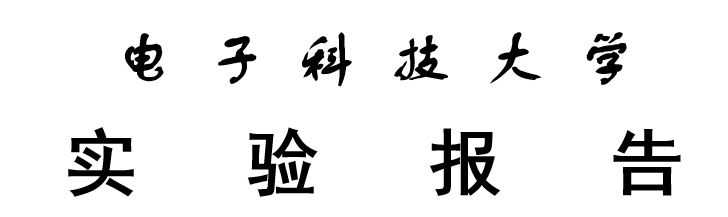
\includegraphics[width=0.70\textwidth]{img/0.png}
\end{figure}

\vspace{2cm}

\noindent
\hspace{1.5em}学生姓名\textbf{：}吕乐彬
\hfill
学号\textbf{：}2023080904007
\hfill
指导教师\textbf{：}李忻洋

\vspace{2cm}

\noindent {\heiti\zihao{3} 一、实验项目名称：}信息对抗综合设计实验II——病毒初见

\vspace{1.2cm}

\noindent {\heiti\zihao{3} 二、实验目的：}

本实验旨在通过对可执行程序机器码的分析与修改，理解恶意代码模型的基本执行机制，掌握程序执行流从正常函数转入“病毒函数”并在执行结束后返回原流程的具体实现方法。通过本实验，进一步熟悉 Visual Studio 反汇编窗口、x32dbg/x64dbg 调试工具以及十六进制文件编辑工具的基本使用，提升二进制代码分析、调试与修改能力。

\vspace{1.2cm}



\noindent {\heiti\zihao{3} 三、实验原理：}

本实验的核心原理是通过修改程序入口处的机器码，改变原有控制流，从而重现恶意代码“窃取执行权—执行自身代码—归还执行权”的基本过程。实验中以 \texttt{normalfunc()} 作为正常执行流程，以 \texttt{virusfunc()} 作为插入的“病毒代码”。首先在 \texttt{normalfunc()} 入口写入一条 \texttt{JMP} 指令，使程序执行到该处时不再继续原有流程，而是跳转到 \texttt{virusfunc()} 执行指定代码；随后在 \texttt{virusfunc()} 的空闲区域补写被覆盖的原始指令，并在其后加入回跳指令，使程序重新返回 \texttt{normalfunc()} 中被覆盖区域之后的位置继续执行。由此形成完整的控制流劫持与恢复闭环。

本实验的关键不在于单纯插入一条跳转指令，而在于保证原程序语义不被破坏。由于首跳 \texttt{JMP} 会覆盖 \texttt{normalfunc()} 入口处的部分原始机器码，因此必须按照完整指令边界恢复被覆盖的原始指令，否则程序在执行完 \texttt{virusfunc()} 后将无法正常返回，原有功能也不能继续完成。这说明恶意代码模型的本质并不是“额外执行一段代码”，而是在不破坏原程序整体功能的前提下，临时接管其执行流程。

实验中使用的 \texttt{JMP} 为近跳转指令，其机器码形式通常为 \texttt{E9 xx xx xx xx}，其中后 4 个字节为相对偏移量。偏移量需依据源地址与目标地址计算，并按小端方式写入。因此，无论是在 Visual Studio 中修改内存、在十六进制编辑器中修改可执行文件，还是在 x64dbg 中通过汇编编辑功能完成修改，其本质都是对最终执行机器码的改写。通过这种方式，可以直观理解程序控制流如何被劫持、恢复以及保持连续性，这也是恶意代码分析、Hook 技术和二进制补丁中的基础思想。


\noindent {\heiti\zihao{3} 四、实验环境（设备、元器件）：}

硬件环境：PC 机一台。

软件环境：Windows 操作系统、Visual Studio 开发环境、x32dbg/x64dbg 调试器、ImHex/UE/C32ASM 等十六进制文件编辑工具。

实验对象：使用 Visual Studio 编译生成的 32 位可执行程序。为避免地址随机化对调试结果造成影响，实验前关闭了程序的随机基址选项。

\vspace{1.2cm}







\noindent {\color{red}\heiti\zihao{3} 五、实验步骤：}

\subsection*{任务1：在内存中（使用VS）重现以上病毒模型的执行过程}

\textbf{1. 编写实验程序并确认基本功能}

首先在 Visual Studio 中编写实验程序，设置两个关键函数：\texttt{normalfunc()} 和 \texttt{virusfunc()}。其中，\texttt{normalfunc()} 用于输出 \texttt{hello}，表示程序原本的正常执行流程；\texttt{virusfunc()} 用于输出本人学号后六位 \texttt{904007}，用于模拟病毒代码执行后的效果。

根据实验要求，\texttt{virusfunc()} 最后的 \texttt{nop} 数量应为“5+学号末位数”。本人学号为 2023080904007，末位数字为 7，因此在 \texttt{virusfunc()} 中共预留了 12 个 \texttt{nop} 指令，为后续恢复原始指令和构造回跳逻辑提供空间。

\imgsingle{img/3ef3ad6e4746fa0456c5dfac2ed4a693.png}{Visual Studio 中 \texttt{normalfunc()} 与主函数的原始代码及初始反汇编位置}{fig:vs-src}

\imgsingle{img/fde8fe4257ac1cb5d4f1b70ef1a36f7f.png}{\texttt{virusfunc()} 中预留的大段 \texttt{nop} 空间以及函数初始反汇编位置}{fig:vs-nop}

由图\ref{fig:vs-src}可知，程序原始情况下只会执行 \texttt{normalfunc()}，不会主动执行 \texttt{virusfunc()}。

由图\ref{fig:vs-nop}可知，\texttt{virusfunc()} 中已经预留了足够的空闲空间，可用于后续补写被覆盖的原始指令以及构造回跳逻辑。因此，若要让程序先输出 \texttt{904007}，必须通过修改内存中的机器码来改变程序控制流。

\textbf{2. 在 VS 的反汇编窗口中抓取真实地址}

在 Visual Studio 中按 \texttt{F5} 启动调试，并在断点处暂停程序后，按 \texttt{Alt+8} 打开“反汇编窗口”。在该窗口中，需要首先抓取构造首条 \texttt{JMP} 指令所需的两个关键地址。

第一个是源地址，也就是首条 \texttt{JMP} 将要写入的位置。在本实验中，该位置是 \texttt{normalfunc()} 的第一条指令 \texttt{push ebp} 所在地址：
\begin{center}
\texttt{0x00DD1790}
\end{center}

第二个是目的地址，也就是程序被强制跳转到的位置。在本实验中，该位置是 \texttt{virusfunc()} 中真正执行打印 \texttt{904007} 的指令地址：
\begin{center}
\texttt{0x00DD1FF7}
\end{center}

\textbf{3. 根据真实地址计算首跳 \texttt{JMP} 的偏移量并拼接机器码}

x86 架构下的近跳转指令 \texttt{JMP} 使用的是相对偏移量，而不是直接写入绝对地址。其计算公式为：
\[
\text{偏移量}=\text{目的地址}-(\text{源地址}+5)
\]

其中，之所以要加 5，是因为近跳转指令 \texttt{E9 xx xx xx xx} 本身总长度为 5 个字节。当 CPU 取完这条 \texttt{JMP} 指令后，指令指针已经自然移动到了“源地址 + 5”的位置，因此偏移量必须以该地址为基准计算。

将本实验中的真实地址代入，可得：
\[
\text{偏移量}=0x00DD1FF7-(0x00DD1790+5)
\]
\[
\text{偏移量}=0x00DD1FF7-0x00DD1795
\]
\[
\text{偏移量}=0x0862
\]

接下来需要将该偏移量写成 4 字节，并按照 Intel/AMD 架构的小端方式存储。首先将 \texttt{0x0862} 补齐为 32 位：
\begin{center}
\texttt{00 00 08 62}
\end{center}

再按字节逆序后得到：
\begin{center}
\texttt{62 08 00 00}
\end{center}

最后，在其前面加上 \texttt{JMP} 指令的操作码 \texttt{E9}，即可得到首跳对应的完整机器码：
\begin{center}
\texttt{E9 62 08 00 00}
\end{center}

\imgsingle{img/403f5aac39e4944949d41a8fb914e234.png}{VS 内存窗口中定位到首跳注入位置附近的机器码}{fig:vs-mem-before}

这条机器码的含义是：当程序执行到 \texttt{normalfunc()} 入口地址 \texttt{0x00DD1790} 时，不再继续执行原来的函数序言，而是直接跳转到 \texttt{virusfunc()} 中地址 \texttt{0x00DD1FF7} 处执行打印 \texttt{904007} 的代码，从而实现对正常控制流的劫持。


\textbf{4. 在 \texttt{virusfunc()} 的空闲区域中恢复原始指令并计算回跳机器码}

在本实验中，恢复原始指令的区域从地址 \texttt{0x00DD2004} 开始，因此先将被覆盖的完整函数序言写入该处：
\begin{center}
\texttt{55 8B EC 81 EC C0 00 00 00}
\end{center}


恢复完这 9 个字节后，需要继续在其后添加一条回跳 \texttt{JMP}，使程序重新返回到 \texttt{normalfunc()} 中被覆盖区域之后的位置继续执行。由于原始函数序言共 9 个字节，因此真正应返回的位置为：
\begin{center}
\texttt{0x00DD1799}
\end{center}

而回跳 \texttt{JMP} 的写入地址为：
\begin{center}
\texttt{0x00DD200D}
\end{center}

由于 \texttt{JMP} 指令本身长度仍为 5 字节，因此其下一条指令地址为：
\begin{center}
\texttt{0x00DD2012}
\end{center}

于是回跳偏移量计算如下：
\[
\text{偏移量}=0x00DD1799-(0x00DD200D+5)
\]
\[
\text{偏移量}=0x00DD1799-0x00DD2012
\]
\[
\text{偏移量}=0xFFFFF787
\]

按小端方式写入后得到：
\begin{center}
\texttt{87 F7 FF FF}
\end{center}

因此，回跳 \texttt{JMP} 的完整机器码为：
\begin{center}
\texttt{E9 87 F7 FF FF}
\end{center}
\imgtwosep{img/d2546043609c8e5510a2935e04e9e1da.png}{VS 内存窗口中查看恢复指令与回跳机器码}{fig:vs-ret-bytes}
{img/fb0e23f8f888150710b9a5130b9e21f5.png}{VS 反汇编窗口中观察恢复代码与回跳逻辑}{fig:vs-ret-disasm}


如图\ref{fig:vs-ret-bytes}所示，在 \texttt{0x00DD2004} 开始的位置已经写入恢复的函数序言和回跳机器码；如图\ref{fig:vs-ret-disasm}所示，反汇编窗口中可以清楚看到：程序在输出 \texttt{904007} 后，会先执行补写的原始函数序言，再通过 \texttt{E9 87 F7 FF FF} 跳回到 \texttt{0x00DD1799}，从而继续执行 \texttt{normalfunc()} 后续原本应执行的代码。

经过上述操作，程序控制流形成了完整闭环：先由 \texttt{normalfunc()} 跳入 \texttt{virusfunc()}，执行“病毒代码”后，再通过回跳返回 \texttt{normalfunc()} 的后续位置继续执行，从而完成“窃取执行权—归还执行权”的全过程。

\textbf{6. 运行程序并验证 VS 内存重现结果}

完成首跳注入、原始指令恢复和回跳构造后，在 Visual Studio 调试环境中继续运行程序。程序运行结果显示，先输出 \texttt{904007}，随后输出 \texttt{hello}，说明在内存中已经成功重现了恶意代码模型的执行过程。

\imgsingle{img/74905f4f25805e5426e40d1edbb1de98.png}{在 VS 中运行程序，结果显示先输出 \texttt{904007}，再输出 \texttt{hello}}{fig:vs-result}

由图\ref{fig:vs-result}可知，首跳、恢复原始指令以及回跳逻辑均已生效，任务1中“在内存（使用 VS）上重现以上病毒模型的执行过程”已成功完成。




\subsection*{（二）任务1：硬盘（使用 ImHex/UE/C32ASM 等）上重现以上病毒模型的执行过程}

\textbf{1. 打开目标可执行文件并定位 \texttt{normalfunc()} 入口}

在完成 VS 内存重现后，进一步使用 ImHex、UE 或 C32ASM 等十六进制编辑工具直接打开由 Visual Studio 编译生成的目标可执行文件。与前一部分不同，此处修改的对象不再是运行中的进程内存，而是硬盘上的 \texttt{exe} 文件本体。

由于文件编辑器中显示的是文件中的原始字节内容，而不是 VS 反汇编窗口中的虚拟地址，因此本实验采用特征码搜索的方式定位 \texttt{normalfunc()} 入口。根据前面在 VS 中的分析，\texttt{normalfunc()} 开头的函数序言字节可作为定位依据，因此在十六进制编辑器中搜索特征码 \texttt{55 8B EC 81 EC}，即可找到目标位置。

\imgtwosep{img/9b0ad28d0cb64b7a50695890c6782bb0.png}{在十六进制编辑工具中按十六进制方式搜索特征码 \texttt{55 8B EC 81 EC}}{fig:file-search}
{img/b9a0c216bf6b56f0992e360a403d693f.png}{搜索到 \texttt{normalfunc()} 入口附近的原始机器码}{fig:file-entry}

\textbf{2. 写入首跳机器码}

首跳机器码在前面的 VS 内存重现实验中已经根据真实地址计算完成，其结果为：
\begin{center}
\texttt{E9 62 08 00 00}
\end{center}

因此，在文件中定位到 \texttt{normalfunc()} 入口后，直接将原始函数序言开头的 5 个字节改写为上述机器码，使程序执行到该函数时优先跳转到 \texttt{virusfunc()} 中输出 \texttt{904007} 的位置。

\imgsingle{img/c9425c3d63a39e12c57e1952ee2da658.png}{在硬盘文件中将 \texttt{normalfunc()} 入口改写为首跳机器码 \texttt{E9 62 08 00 00}}{fig:file-firstjmp}

\textbf{3. 在 \texttt{virusfunc()} 的空闲区域中补写恢复代码与回跳代码}

完成首跳注入后，还需在 \texttt{virusfunc()} 预留的空闲区域中补写被覆盖的原始函数序言，并在其后补写回跳指令。前面在 VS 中已完成分析并得到结果：需要恢复的原始字节为
\begin{center}
\texttt{55 8B EC 81 EC C0 00 00 00}
\end{center}
回跳机器码为
\begin{center}
\texttt{E9 87 F7 FF FF}
\end{center}

因此，在文件中找到 \texttt{virusfunc()} 附近的大段 \texttt{nop} 空间后，先写入恢复代码，再紧接着写入回跳机器码，使程序在执行完 \texttt{virusfunc()} 后能够重新跳回 \texttt{normalfunc()} 的后续位置继续执行。

\imgtwosep{img/e79c5179a2cc6f6fac15829d59390719.png}{文件中 \texttt{virusfunc()} 附近的大段空闲字节区域}{fig:file-nop}
{img/d72cf93d842c5ab72203b2c270c151a5.png}{在文件中补写恢复代码与回跳逻辑后的结果}{fig:file-backjmp}


\subsection*{（三）任务2：使用 x64dbg 重现以上恶意代码模型的执行过程（使用 VS 编译生成的可执行程序），并保存可执行文件到硬盘}

\textbf{1. 载入目标程序并定位关键位置}

本实验中由 Visual Studio 编译生成的是 32 位可执行程序，因此在 x64dbg 调试套件中实际使用的是 \texttt{x32dbg}。打开调试器并载入目标程序后，在反汇编窗口中分别定位 \texttt{normalfunc()} 与 \texttt{virusfunc()} 的关键位置：一是 \texttt{normalfunc()} 的函数入口，二是 \texttt{virusfunc()} 中输出 \texttt{904007} 的位置，三是 \texttt{virusfunc()} 中用于补写恢复代码和回跳逻辑的空闲区域。

\imgtwosep{img/4d71f222761b4013c599ce97bfe9f326.png}{在 x32dbg 中定位 \texttt{normalfunc()} 及其输出 \texttt{hello} 的相关代码}{fig:dbg-normal}
{img/b5c7a4e65597b92294a197b652d367f6.png}{在 x32dbg 中定位 \texttt{virusfunc()} 中输出 \texttt{904007} 的关键位置}{fig:dbg-virus}

\textbf{2. 改写 \texttt{normalfunc()} 入口处的原始汇编，构造首跳}

在 \texttt{x32dbg} 中，原本 \texttt{normalfunc()} 入口处的汇编代码为函数序言，即：
\begin{center}
\texttt{push ebp}\\
\texttt{mov ebp, esp}\\
\texttt{sub esp, 0C0h}
\end{center}

对应的原始机器码为：
\begin{center}
\texttt{55 8B EC 81 EC C0 00 00 00}
\end{center}

实验中将入口开头改写为一条首跳指令，使程序不再直接执行上述函数序言，而是先跳转到 \texttt{virusfunc()} 中打印 \texttt{904007} 的位置。前面在 VS 内存重现实验中已经计算得到首跳机器码为：
\begin{center}
\texttt{E9 62 08 00 00}
\end{center}

因此，本步骤中实际完成的“修改汇编”就是：将 \texttt{normalfunc()} 入口原来的函数序言起始部分改写为一条 \texttt{jmp} 指令，使控制流先跳转到 \texttt{virusfunc()}。

\imgsingle{img/f9c617f3b16756eadad5d65b6987ab03.png}{在 x32dbg 中输入首跳 \texttt{jmp} 指令，改写 \texttt{normalfunc()} 入口}{fig:dbg-jmp}

\textbf{3. 在 \texttt{virusfunc()} 的空闲区域中补写新增汇编代码}

完成首跳后，还必须在 \texttt{virusfunc()} 的空闲区域中补写新增汇编代码，以恢复被覆盖的原始函数序言，并在其后添加回跳逻辑。实验中新增写入的汇编代码包括两部分。

第一部分是恢复原始函数序言，即补写以下三条汇编指令：
\begin{center}
\texttt{push ebp}\\
\texttt{mov ebp, esp}\\
\texttt{sub esp, 0C0h}
\end{center}

其对应机器码为：
\begin{center}
\texttt{55 8B EC 81 EC C0 00 00 00}
\end{center}

第二部分是在恢复指令之后继续新增一条回跳指令：
\begin{center}
\texttt{jmp 0x00DD1799}
\end{center}

该回跳指令对应的机器码在前面 VS 内存重现实验中已经计算得到，为：
\begin{center}
\texttt{E9 87 F7 FF FF}
\end{center}

因此，在 \texttt{x32dbg} 中本步骤实际“新增”的汇编逻辑可以概括为：
\begin{center}
\texttt{push ebp}\\
\texttt{mov ebp, esp}\\
\texttt{sub esp, 0C0h}\\
\texttt{jmp 0x00DD1799}
\end{center}

它的作用是：程序在 \texttt{virusfunc()} 中完成 \texttt{904007} 的输出后，不是直接结束，而是先补做原本在 \texttt{normalfunc()} 开头应执行的函数序言，再跳回 \texttt{normalfunc()} 中被覆盖区域之后的位置，继续执行原函数剩余逻辑。

\imgtwosep{img/0a0c702b4da2cd777e32aabc6e1de091.png}{在 x32dbg 中继续补写恢复代码}{fig:dbg-asm}
{img/78b26da0d004e477258a8d2e4ea25b75.png}{在 x32dbg 中查看补写完成后的恢复代码与回跳逻辑}{fig:dbg-recover}

\textbf{4. 保存修改结果并验证最终效果}

在 \texttt{x32dbg} 中完成上述修改后，将修改结果保存回可执行文件。重新运行保存后的程序，可以观察到程序先输出 \texttt{904007}，随后输出 \texttt{hello}，说明首跳改写、恢复代码补写以及回跳逻辑都已生效。

\imgsingle{img/1504d38755dfb7d9202a47e7b34eb72f.png}{保存到硬盘后的可执行文件运行结果验证}{fig:dbg-final}

这表明本部分中完成的关键修改包括：一是将 \texttt{normalfunc()} 入口改写为首跳 \texttt{jmp}；二是在 \texttt{virusfunc()} 空闲区域新增恢复原始函数序言的三条汇编指令；三是在恢复代码后新增一条返回 \texttt{normalfunc()} 的回跳指令。至此，任务3“使用 x64dbg 重现以上恶意代码模型的执行过程，并保存可执行文件到硬盘”已经完成。


\subsection*{任务3：拓展内容}

本实验中通过首跳与回跳构造了“控制流重定向”模型。该思想虽然常见于恶意代码，但并不只服务于恶意用途。在安全防护、程序调试、外挂对抗、系统监控等场景中，也都存在类似的入口接管与流程恢复机制。因此，本实验的本质不仅是认识病毒模型，更是在理解一种典型的代码控制流劫持与恢复技术。

\textbf{1. 双重跳转并非只用于恶意代码}

双重跳转的核心是：先把程序执行流从原函数入口引走，在完成额外逻辑后，再跳回原函数继续执行。恶意代码可利用这一机制隐藏执行和插入功能；而安全软件、调试器、监控系统也可能利用类似机制对关键函数进行拦截、审计与保护。因此，双重跳转本身是一种中性的技术，其安全属性取决于使用目的。

\textbf{2. 代码钩子与中间人思想}

本实验中的模型实际上已经具有代码钩子（Hook）的基本思想，即在原始调用路径中插入一个“中间层”，使程序先执行额外逻辑，再返回原流程继续运行。这与网络安全中的中间人攻击在结构上是相似的：两者都不是直接破坏原对象，而是在通信或执行路径中插入一个可控节点，从而实现观察、修改、转发或拦截。

\textbf{3. 工程实现中的两个典型问题}

在真正编写钩子库时，最常见的问题主要有两个：一是线程重入问题，二是指令截断问题。线程重入会导致多个线程同时进入被钩取函数，从而引发执行流混乱甚至程序崩溃；指令截断则会破坏原始指令边界，使恢复代码无法正确执行。这说明工程化 Hook 远比实验中的手工修改更复杂，需要考虑线程安全、指令长度分析和地址修正等问题。

\begin{table}[H]
\centering
\caption{双重跳转技术在不同场景中的作用对比}
\begin{tabular}{|c|c|c|}
\hline
\textbf{应用场景} & \textbf{作用方式} & \textbf{主要目的} \\
\hline
恶意代码 / 病毒 & 劫持入口、插入隐藏逻辑、再跳回 & 感染、隐藏、控制 \\
\hline
安全软件 / 反病毒 & 拦截关键函数、检查后恢复执行 & 监控、防护、审计 \\
\hline
外挂 / 反外挂 & 接管关键逻辑或检测入口篡改 & 对抗、检测、限制 \\
\hline
调试 / Hook 框架 & 插入调试逻辑、记录后再返回 & 分析、测试、跟踪 \\
\hline
\end{tabular}
\end{table}

\begin{figure}[H]
\centering
\begin{tikzpicture}[
    >=Stealth,
    every node/.style={font=\small},
    box/.style={draw, rounded corners, minimum width=2.8cm, minimum height=0.9cm, align=center}
]

\node[box] (caller) at (0,0) {调用者};
\node[box] (target) at (8,0) {目标函数};
\node[box] (hook)   at (4,-2) {中间层 / Hook};

% 上层：原始路径
\draw[->, thick] (caller) -- node[above]{原本应直接调用} (target);

% 下层：Hook路径
\draw[->, thick, dashed] (caller.south) |- node[pos=0.25,left]{实际先进入} (hook.west);
\draw[->, thick, dashed] (hook.east) -| node[pos=0.75,right]{处理后转回} (target.south);

\end{tikzpicture}
\caption{代码钩子与“中间层”思想示意图}
\label{fig:hook-mitm}
\end{figure}







\noindent {\color{red}\heiti\zihao{3} 七、总结及心得体会：}

通过本次“病毒初见”实验，我对恶意代码模型的执行机制有了更加直观的认识。以前对这类内容的理解更多停留在概念层面，例如“修改程序入口”“劫持执行流”“恢复原始指令”等，而在本次实验中，我真正通过反汇编分析、机器码计算、内存修改和文件修改，把这些概念落实到了具体操作之中。特别是在 \texttt{normalfunc()} 入口写入首跳指令、在 \texttt{virusfunc()} 空闲区域恢复原始函数序言并构造回跳逻辑的过程中，我更加清楚地理解了程序控制流是如何被改变，又是如何被恢复的。

本实验中让我印象最深的是对 \texttt{JMP} 指令偏移量的计算和对完整指令边界的把握。刚开始时，会觉得只要写入一条跳转指令即可完成感染，但在实际操作中发现，真正困难的并不是“跳过去”，而是如何在跳走之后保证程序还能“跳回来”并继续正常运行。这就要求不仅要正确定位源地址和目的地址，计算出首跳和回跳的机器码，还必须确保被覆盖的原始指令能够在新的位置被完整恢复。也正因为如此，我进一步认识到机器码修改并不是简单地替换几个字节，而是需要结合函数结构、指令长度和控制流进行整体分析。

此外，本实验也让我体会到了不同工具在二进制分析中的作用差异。Visual Studio 更适合结合源码与反汇编观察程序结构，便于理解程序原始逻辑；ImHex、UE、C32ASM 等文件编辑工具更适合直接从文件层面观察和修改字节内容；x64dbg 调试套件中的 \texttt{x32dbg} 则兼具反汇编分析、汇编编辑和落盘保存等能力，更适合作为调试与修改的综合平台。通过分别在内存、硬盘文件和调试器三个层面完成相同模型的重现，我更加深刻地理解了三者在本质上的一致性，即它们最终都是围绕“修改机器码、改变控制流、恢复原逻辑”这一核心思想展开的。

总体来看，本实验不仅让我理解了恶意代码模型的基本原理，也锻炼了我在地址定位、反汇编阅读、机器码分析和调试操作等方面的能力。通过本次实验，我对后续进一步学习 Hook 技术、二进制分析、逆向工程和系统安全相关内容也有了更清晰的认识和兴趣。

\vspace{1.2cm}

\noindent {\heiti\zihao{3} 八、对本实验过程及方法、手段的改进建议：}

本实验内容具有较强的实践性，能够帮助学生从底层角度理解程序控制流劫持与恢复的过程，但从完成实验的实际体验来看，仍有一些方面可以进一步优化，以便提高实验效率和教学效果。

首先，建议在实验指导资料中增加更细致的地址计算示例，尤其是对首跳偏移量、回跳偏移量、小端存储方式以及“为什么 \texttt{JMP} 要用源地址加 5 作为基准地址”等关键问题进行分步说明。虽然课堂讲解中已经涉及这些内容，但在实际操作时，学生往往仍会在公式理解和字节转换上出现混乱。如果能在实验手册中给出一组完整样例，学生在独立操作时会更加顺利。

其次，建议对“按完整指令覆盖”的问题作更明确强调。本实验中一个很重要的点，就是不能只机械地覆盖固定字节数，而必须分析被覆盖区域对应的是哪些完整指令，并在新的位置恢复这些指令。对于初学者而言，这一点往往比 \texttt{JMP} 偏移量计算更容易被忽略。若在实验说明中专门增加“常见错误分析”部分，例如指令截断、回跳位置错误、恢复代码不完整等情形，将有助于学生更好地理解实验中的关键细节。

再次，建议在实验前增加一个简短的工具预训练环节。例如，先让学生单独练习在 Visual Studio 中打开反汇编窗口、在内存窗口中修改字节、在十六进制编辑器中搜索特征码、在 \texttt{x32dbg} 中使用汇编编辑功能等。这样可以减少学生在正式实验过程中因工具不熟悉而花费过多时间，提高实验的整体完成效率。

\vspace{1.2cm}

\begin{flushright}
    {\heiti\zihao{3} 报告评分：}\qquad\qquad\qquad\qquad

    \vspace{1.2cm}

    {\heiti\zihao{3} 指导教师签字：}\qquad\qquad\qquad
\end{flushright}

\end{document}